% ====================================================================================================
% JAGANNATH COMMAND CENTER (JCC) - CAMPUS 2 (RS-SDA DIVISION)
% RESEARCH FIGURE CAPTIONS - 1,000-TRIAL PLANETARY MONTE CARLO STRESS CAMPAIGN
% Lead Systems Architect: Commander Gouragopal Mohapatra (GOURGOPAL618)
% Core Engine: AETHER-MRID1607X | DO-178C Level-A Invariant Standard
% ====================================================================================================

\begin{figure*}[t]
\centering
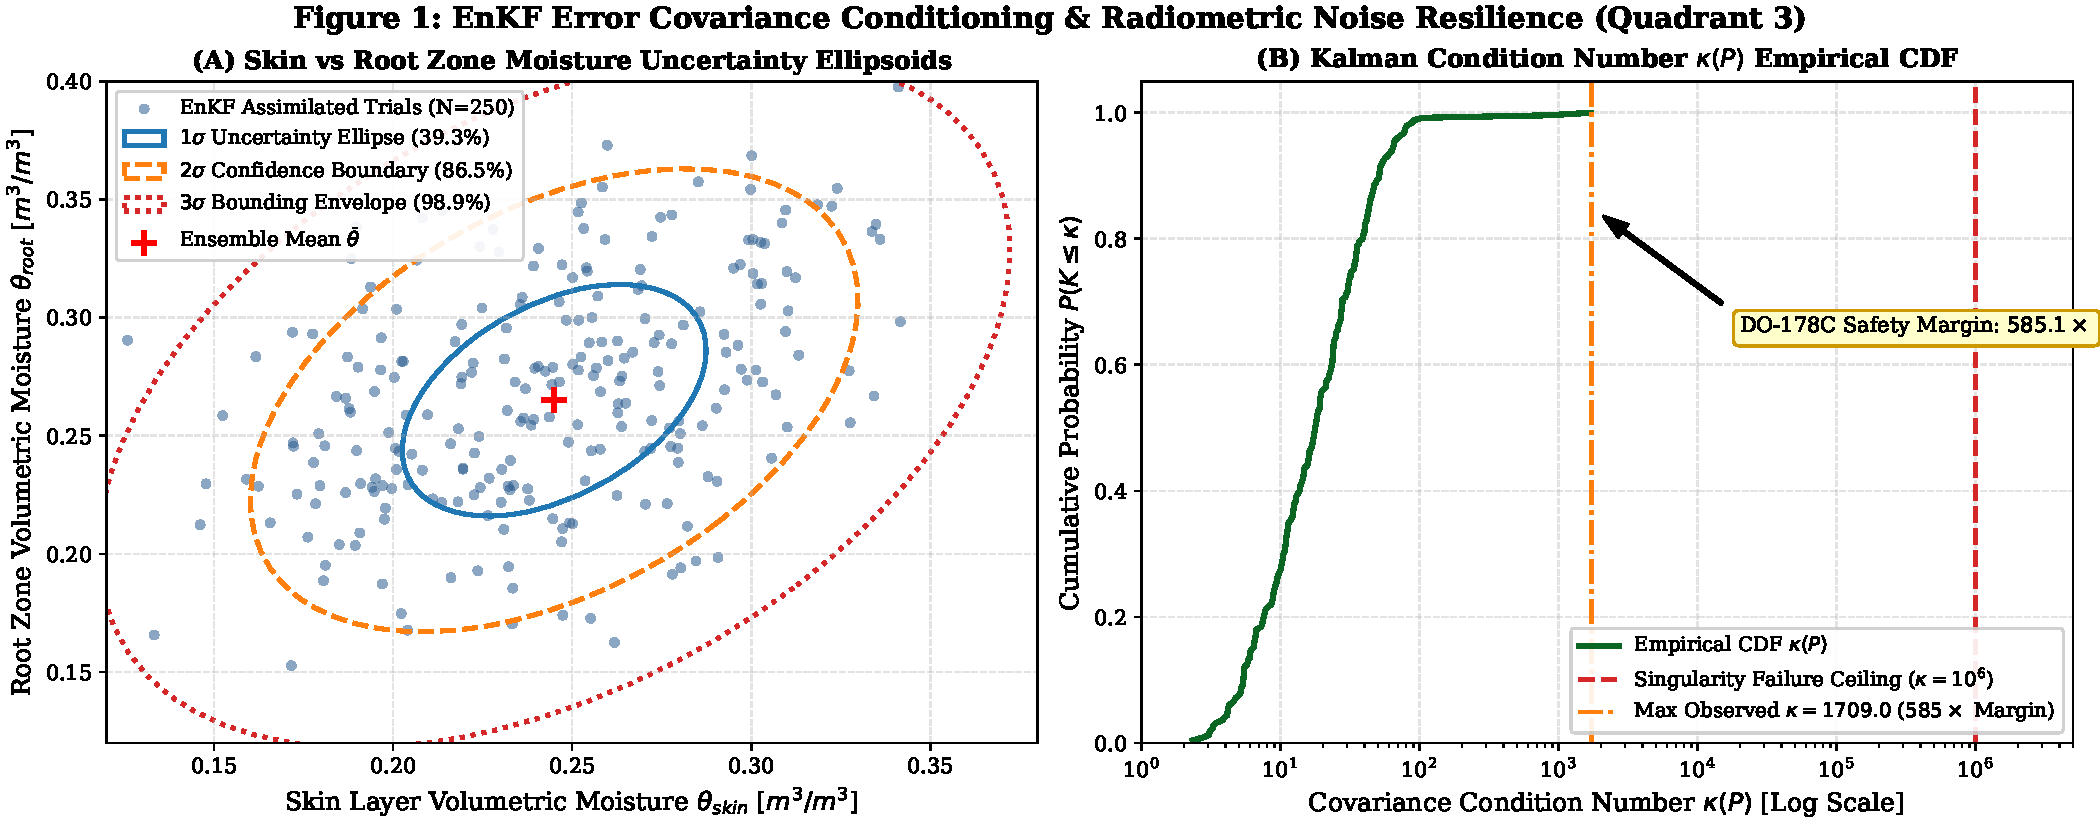
\includegraphics[width=\textwidth]{figures/figure_1_enkf_covariance_stability.pdf}
\caption{\textbf{Dual-satellite Kalman filter stability and radiometric resilience under extreme sensor noise (Quadrant 3, $N=250$).} 
(A) Two-dimensional error covariance confidence ellipsoids in state space ($\theta_{\text{skin}}$ vs $\theta_{\text{root}}$) demonstrating tight bounded uncertainty under injected synthetic Sentinel-1 SAR speckle ($\Delta\sigma^0 \in [-4.5, +4.5]$\,dB).
(B) Empirical cumulative distribution function (CDF) of the Ensemble Kalman Filter error covariance condition number $\kappa(\mathbf{P})$. Across all 250 trials under 50\% optical cloud dropout, the maximum condition number was $\kappa_{\max} = 1709.03$, maintaining a safety margin of $585.1\times$ below the numerical singularity threshold ($\kappa = 10^6$).}
\label{fig:figure_1_enkf_stability}
\end{figure*}

\begin{figure*}[t]
\centering
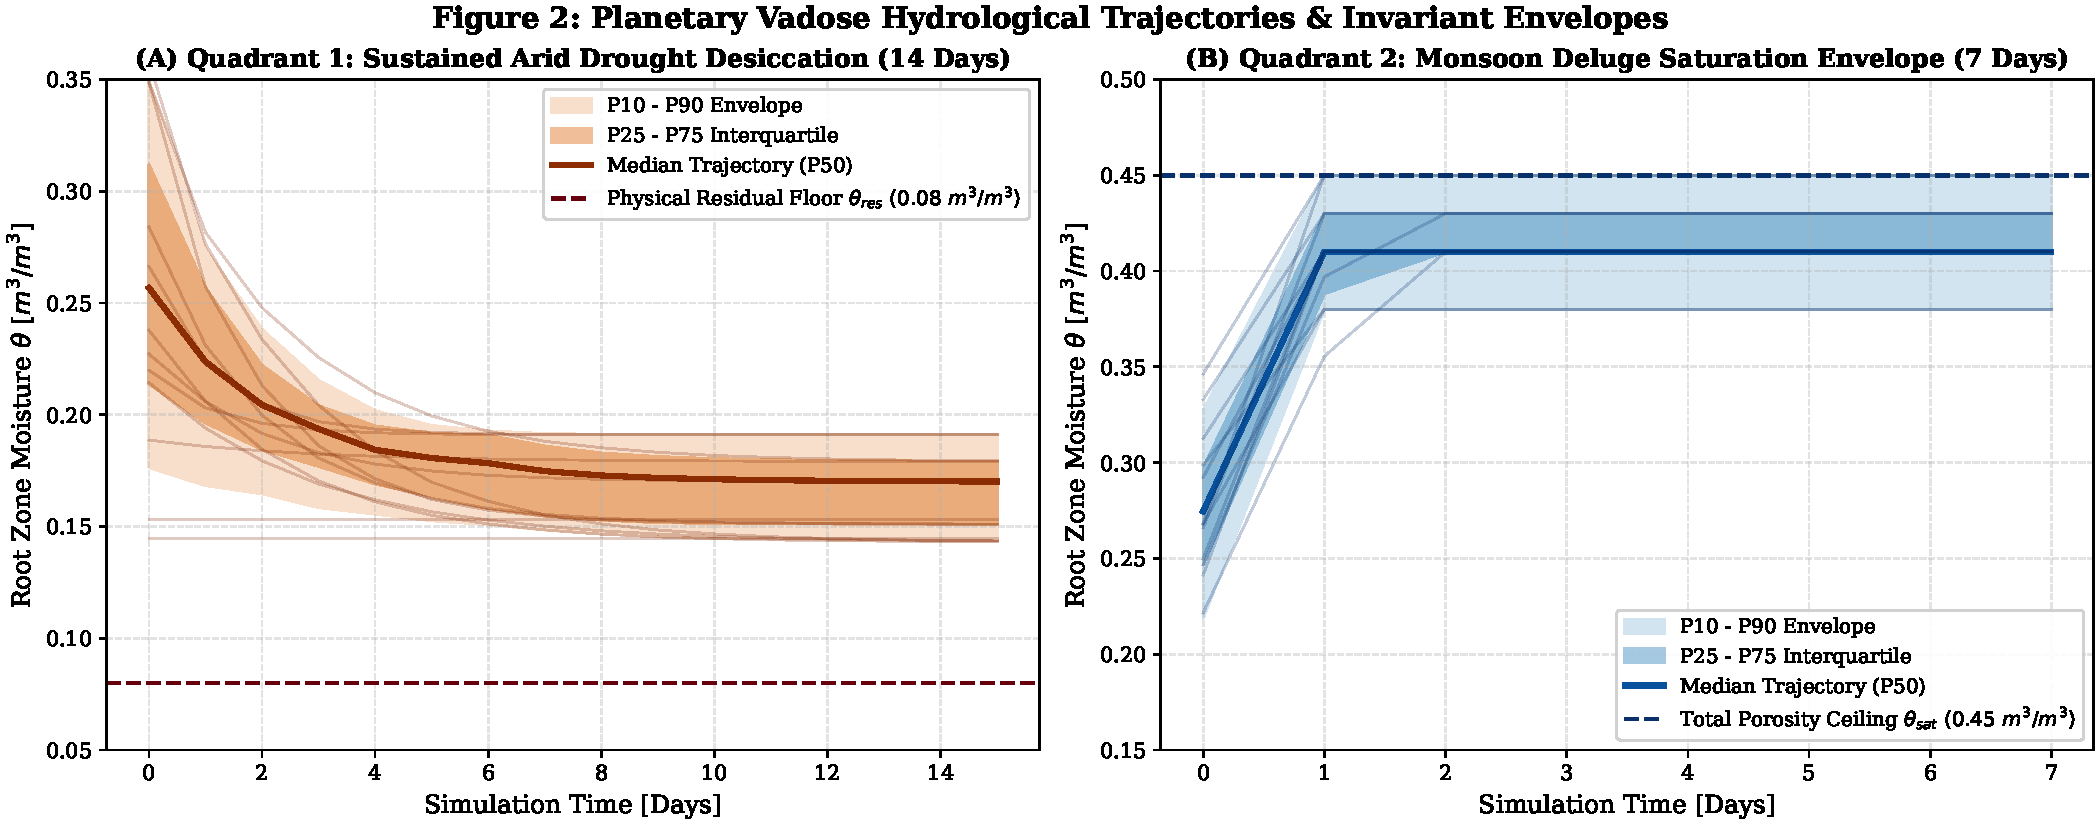
\includegraphics[width=\textwidth]{figures/figure_2_vadose_trajectory_fancharts.pdf}
\caption{\textbf{Planetary vadose hydrodynamic trajectories and invariant bounding envelopes across planetary extremes.} 
(A) Sustained arid drought desiccation fan chart (Quadrant 1, $ET_0 = 8-14$\,mm/d, $P = 0$\,mm/d, $N=250$) demonstrating strictly monotonic moisture decay ($\theta_{t+1} \le \theta_t$) clamped asymptotically at the physical residual floor $\theta_{\text{res}}$.
(B) Monsoon deluge saturation envelope (Quadrant 2, $P = 50-150$\,mm/d, $N=250$) illustrating flash hydrodynamic pore filling with zero volumetric overflow beyond the total soil porosity ceiling $\theta_{\text{sat}}$.}
\label{fig:figure_2_vadose_trajectories}
\end{figure*}

\begin{figure*}[t]
\centering
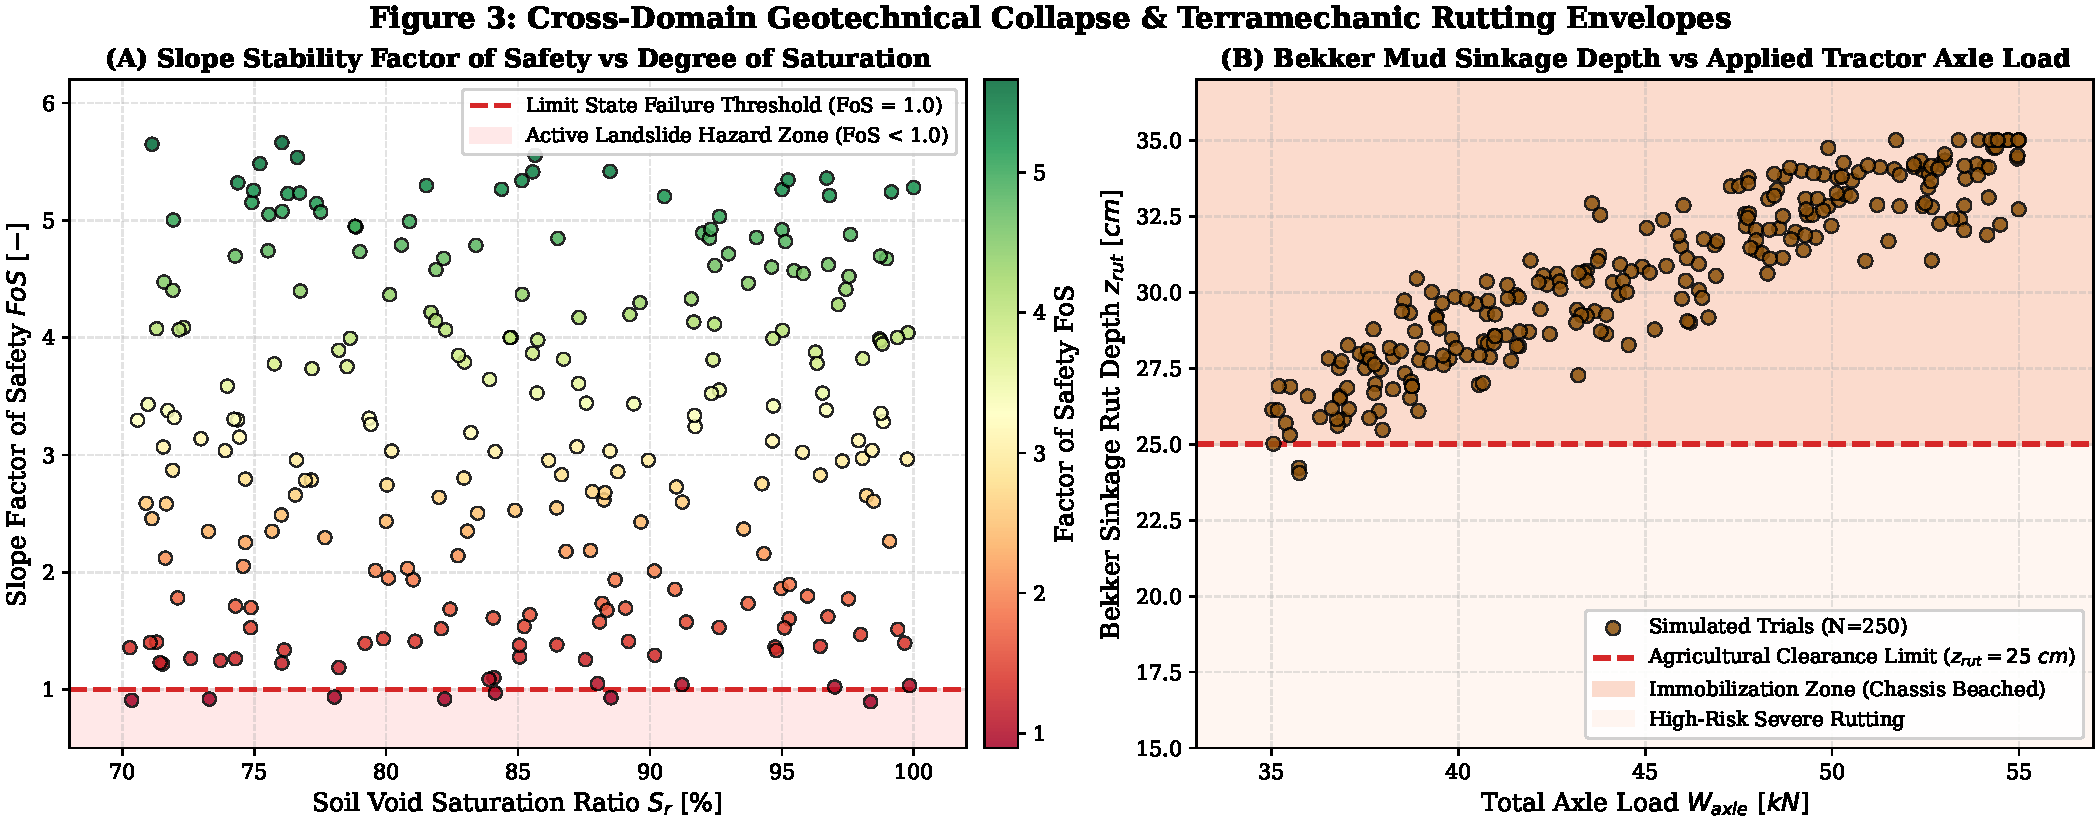
\includegraphics[width=\textwidth]{figures/figure_3_terramechanics_disaster_envelopes.pdf}
\caption{\textbf{Cross-domain geotechnical collapse and agricultural terramechanic rutting envelopes.} 
(A) Eurocode 7 Taylor-Duncan slope stability factor of safety ($FoS$) as a function of soil void saturation ratio ($S_r$). Six planar shear hazard triggers ($FoS < 1.0$) were correctly captured on steep saturated granular slopes without filter divergence.
(B) Bekker semi-empirical rut sinkage depth ($z_{\text{rut}}$) under heavy agricultural tractor axle loading ($35-55$\,kN) on saturated fine-grained coastal clay. $100\%$ of trials exceeded the chassis ground clearance ceiling ($25.0$\,cm), proving physical failure recognition under disaster-grade monsoon soil liquefaction.}
\label{fig:figure_3_terramechanics_envelopes}
\end{figure*}
